%%%%%%%%%%%%%%%%%%%%%%%%%%%%%%%%%%%%%%%%%
% Beamer Presentation
% LaTeX Template
% Version 1.0 (10/11/12)
%
% This template has been downloaded from:
% http://www.LaTeXTemplates.com
%
% License:
% CC BY-NC-SA 3.0 (http://creativecommons.org/licenses/by-nc-sa/3.0/)
%
%%%%%%%%%%%%%%%%%%%%%%%%%%%%%%%%%%%%%%%%%

%----------------------------------------------------------------------------------------
%	PACKAGES AND THEMES
%----------------------------------------------------------------------------------------

\documentclass{beamer}

\mode<presentation> {

% The Beamer class comes with a number of default slide themes
% which change the colors and layouts of slides. Below this is a list
% of all the themes, uncomment each in turn to see what they look like.

%\usetheme{default}
%\usetheme{AnnArbor}
%\usetheme{Antibes}
%\usetheme{Bergen}
\usetheme{Berkeley}
%\usetheme{Berlin}
%\usetheme{Boadilla}
%\usetheme{CambridgeUS}
%\usetheme{Copenhagen}
%\usetheme{Darmstadt}
%\usetheme{Dresden}
%\usetheme{Frankfurt}
%\usetheme{Goettingen}
%\usetheme{Hannover}
%\usetheme{Ilmenau}
%\usetheme{JuanLesPins}
%\usetheme{Luebeck}
%\usetheme{Madrid}
%\usetheme{Malmoe}
%\usetheme{Marburg}
%\usetheme{Montpellier}
%\usetheme{PaloAlto}
%\usetheme{Pittsburgh}
%\usetheme{Rochester}
%\usetheme{Singapore}
%\usetheme{Szeged}
%\usetheme{Warsaw}

% As well as themes, the Beamer class has a number of color themes
% for any slide theme. Uncomment each of these in turn to see how it
% changes the colors of your current slide theme.

%\usecolortheme{albatross}
%\usecolortheme{beaver}
%\usecolortheme{beetle}
%\usecolortheme{crane}
%\usecolortheme{dolphin}
%\usecolortheme{dove}
%\usecolortheme{fly}
%\usecolortheme{lily}
%\usecolortheme{orchid}
%\usecolortheme{rose}
%\usecolortheme{seagull}
%\usecolortheme{seahorse}
%\usecolortheme{whale}
%\usecolortheme{wolverine}

%\setbeamertemplate{footline} % To remove the footer line in all slides uncomment this line
%\setbeamertemplate{footline}[page number] % To replace the footer line in all slides with a simple slide count uncomment this line

%\setbeamertemplate{navigation symbols}{} % To remove the navigation symbols from the bottom of all slides uncomment this line
}
\usepackage{setspace}
\usepackage{graphicx} % Allows including images
\usepackage{booktabs} % Allows the use of \toprule, \midrule and \bottomrule in tables
\setbeamertemplate{caption}[numbered]
%----------------------------------------------------------------------------------------
%	TITLE PAGE
%----------------------------------------------------------------------------------------

\title[]{Loop Acceleration For Tightly-Coupled CPU+FPGA System} 
\author[]{
    Cheng Liu 
    \\Supervisor: Dr. Hayden Kwok-Hay So 
    \\Co-supervisor: Dr. Ngai Wong}
\institute {
    Department of Electrical and Electronic Engineering 
    \\The University of Hong Kong
\medskip
}
\date{\today} % Date, can be changed to a custom date

\graphicspath{{./figures/}} 
\begin{document}

\begin{frame}
\titlepage % Print the title page as the first slide
\end{frame}

%----------------------------------------------------------------------------------------
%	PRESENTATION SLIDES
%----------------------------------------------------------------------------------------

%------------------------------------------------
\section{Background} 
%------------------------------------------------
\begin{frame}[t]
\frametitle{FPGA vs. CPU vs. GPU}
\textbf{FPGA has competitive computation capability and \\
        energy efficiency.} 

\begin{figure}
  \vspace{-1em}
  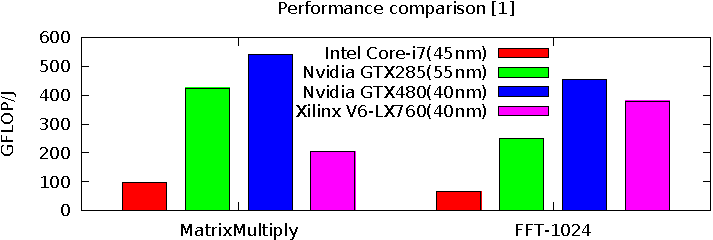
\includegraphics[width=.8\linewidth]{performance-cpu-fpga-gpu}
  \vspace{-1em}
\end{figure}
\begin{figure}
  \vspace{-1em}
  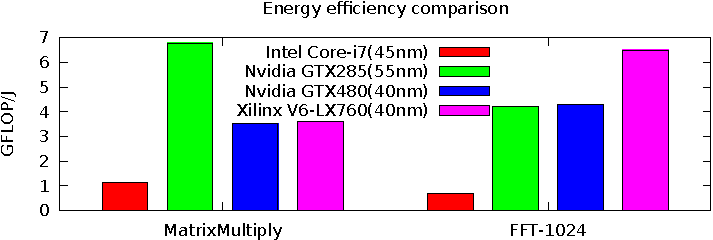
\includegraphics[width=.8\linewidth]{energy-cpu-fpga-gpu}
  \vspace{-1em}
\end{figure}

\begin{spacing}{1.2}
\tiny{[1] Eric S. Chung, etc., Single-Chip Heterogeneous Computing: Does the future include customized
logic, FPGA and GPGPUs?, IEEE International Symposium of Microarchitecture, 2010}
\end{spacing}

\end{frame}

%------------------------------------------------
\begin{frame}[t]

\frametitle{Why isn't FPGA the mainstream computing device?}
\textbf{Main obstacles}
\begin{itemize}

\item High barrier-to-entry
\begin{itemize}
\item Require extensive hardware knowledge,
\item while software engineers usually don't have.
\item ...
\end{itemize}

\item Low design productivity
\begin{itemize}
\item Low level abstraction and long development time
\item Long compilation and implementation time
\item Poor portability and design reuse
\item Difficult to support complex software like OS
\item ...
\end{itemize}

\end{itemize}

\end{frame}

%------------------------------------------------
\section{Related work}
%------------------------------------------------
\begin{frame}[t]
\frametitle{What has the community done to overcome the obstacles?}

\textbf{Design methodologies}
\begin{itemize}
\item High level synthesis languages and tools \\
\footnotesize
Vivado(Xpilot, AutoESL), LegUP, Impulse-C, ...
\normalsize
\item Virtual overlay on top of commerical FPGA \\
\footnotesize 
VirtualRC, Soft coarse-grained reconfigurale array (SCGRA), ...
\normalsize

\end{itemize}

\textbf{CPU+FPGA based hybrid computation}
\begin{itemize}
\item Hybrid computation architectures \\
\footnotesize
Embedded softcore+FPGA, Embedded hardcore+FPGA, General CPU+FPGA, ...
\normalsize
\item Communication libraries, unified memory interfaces, and integrated environments \\
\footnotesize
CoRAM, LEAP, ...
\normalsize
\end{itemize}

\end{frame}

%------------------------------------------------
\begin{frame}[t]
\frametitle{Differences and relations of the design methodologies}

\begin{figure}
\vspace{-1em}
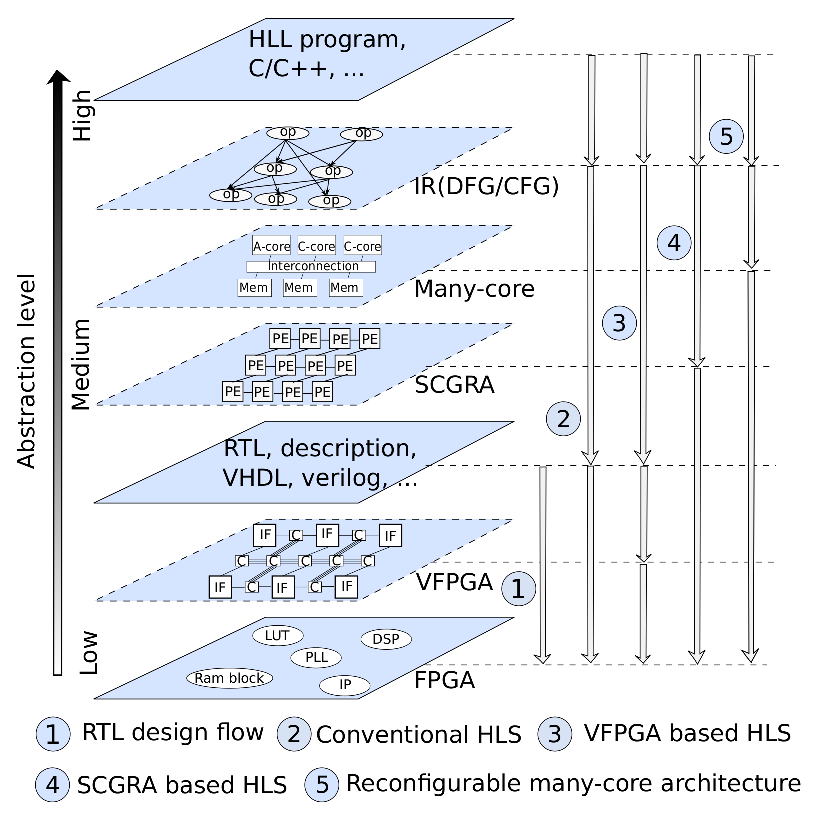
\includegraphics[width=.9\linewidth]{virtual-overlay}
\end{figure}

\end{frame}

%------------------------------------------------
\begin{frame}[t]

\frametitle{Performance vs. productivity vs. overhead}
\begin{figure}
\vspace{-1em}
\includegraphics[width=0.7\linewidth]{performance-vs-productivity-vs-overhead}
\end{figure}

Why SCGRA based HLS has potential to provide better performance?\\
performance = operations per cycle $\times$ \textbf{implementation frequency}

\end{frame}

%------------------------------------------------
\begin{frame}[t]
\frametitle{CPU+FPGA based hybrid computation}

\textbf{Hardware/software co-design}
\begin{figure}
\includegraphics[width=0.8\linewidth]{codesign}
\end{figure}

\textbf{Loop and computation kernel}
\begin{itemize}
\item Most algorithms are implemented following a sequential programming model.
\item Loops are typical computation kernels with large parallel operations.
\end{itemize}

\end{frame}

%------------------------------------------------
\begin{frame}[t]
\frametitle{CPU+FPGA based hyrbid computation architecture}

\begin{figure}
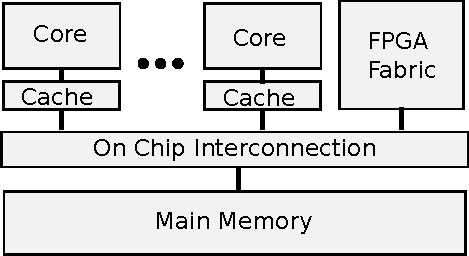
\includegraphics[width=0.5\linewidth]{system-context}
\vspace{-1em}
\caption{Single chip multicore with FPGA accelerator}
\end{figure}

\begin{figure}
\includegraphics[width=0.5\linewidth]{system-context2}
\vspace{-1em}
\caption{Shared memory multiprocessor with FPGA accelerator}
\end{figure}

\end{frame}

%------------------------------------------------
\begin{frame}[t]
\frametitle{Previous SCGRA Work}
\textbf{What have been done?}
\begin{itemize}
\item Introduced the SCGRA layer for HLS,
\item showed potential design productivity improvement,
\item and proved its energy efficiency using an application specific SCGRA topology
\end{itemize}
\textbf{What are still missing?}
\begin{itemize}
\item The relationship between a holistic loop and its kernel data flow graph,
\item influence of the communication between CPU and FPGA on the SCGRA based HLS.
\end{itemize}
\end{frame}

%------------------------------------------------
\begin{frame}[t]
\frametitle{Main goal of this work}
\textbf{Accelerate loop on a CPU+FPGA system}
\begin{itemize}
\item Optimal loop unrolling for the SCGRA based accelerator
\item Application specific on-chip buffering including data prefetching and buffer structure
customization 
\end{itemize}

\end{frame}

%------------------------------------------------
\section{Research scheme}
%------------------------------------------------
\begin{frame}[t]
\frametitle{Hardware infrastructure} 
\textbf{SCGRA based CPU+FPGA accelerator}
\begin{figure}
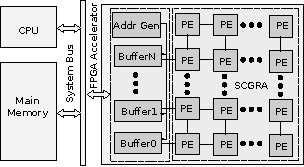
\includegraphics[width=0.65\linewidth]{scgra-acceleratorv2}
\end{figure}

\textbf{Softness of the accelerator}
\begin{itemize}
\item SCGRA structure could be reconfigurable
\item On chip buffer could be reconfigurable
\end{itemize}
\end{frame}

%------------------------------------------------
\begin{frame}[t]
\frametitle{SCGRA based accelerator design flow}

\begin{figure}
\vspace{-1em}
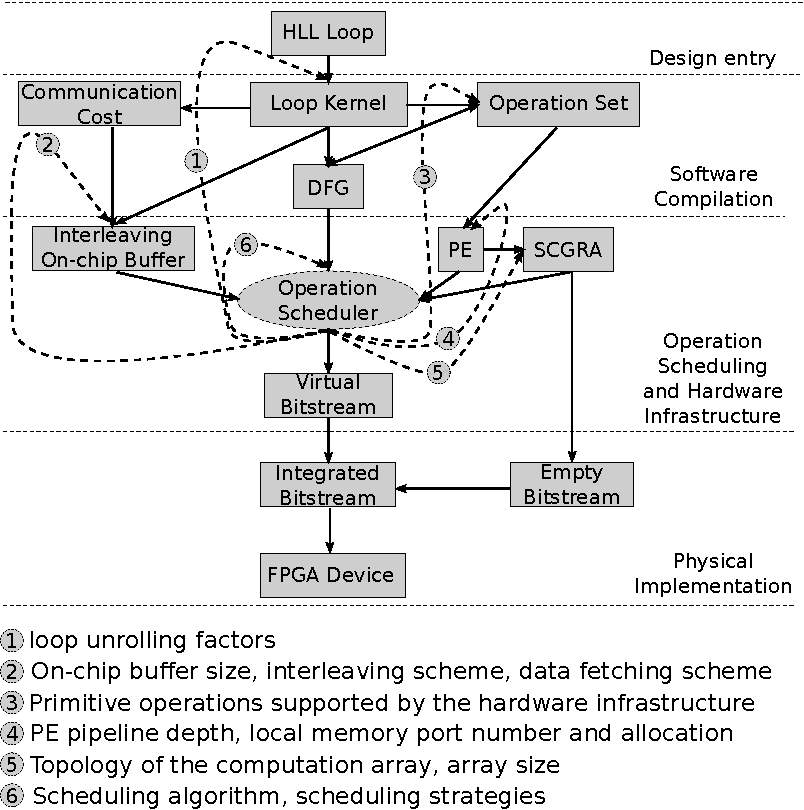
\includegraphics[width=0.76\linewidth]{design-space-overview2}
\end{figure}

\end{frame}

%------------------------------------------------
\begin{frame}[t]
\frametitle{Optimal loop unrolling}

\textbf{Why loop unrolling and why not fully unroll the loop?}
\begin{itemize}
\item Increases parallel operations and improves performance
\item Induces larger hardware overhead performance 
\item Benefit may be limited by system constrains.
\end{itemize}

\textbf{Simplified loop unrolling}
\begin{figure}
\vspace{-1em}
\includegraphics[width=0.95\linewidth]{system-loop-unrolling}
\end{figure}

\end{frame}

%------------------------------------------------
\begin{frame}[t]
\frametitle{On-chip buffering}

\begin{figure}
\vspace{-1em}
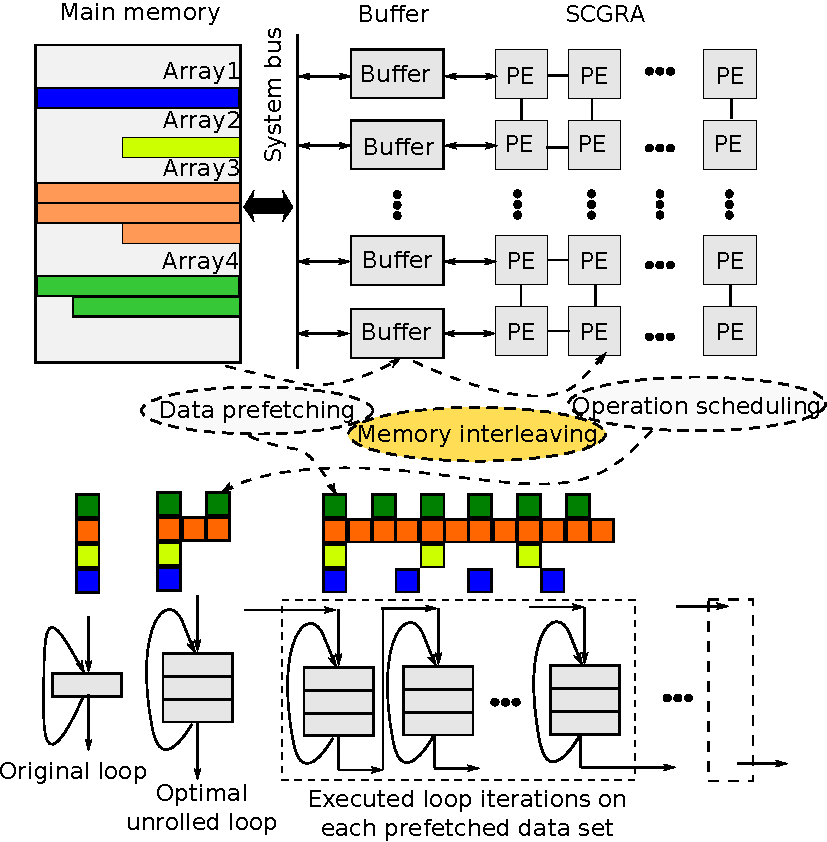
\includegraphics[width=0.7\linewidth]{on-chip-buffer}
\end{figure}

\end{frame}

%------------------------------------------------
\section{Current progress}
\begin{frame}[t]
\frametitle{Quantify the productivity of the SCGRA based HLS}
\textbf{Current SCGRA based HLS}
\begin{figure}
\vspace{-1em}
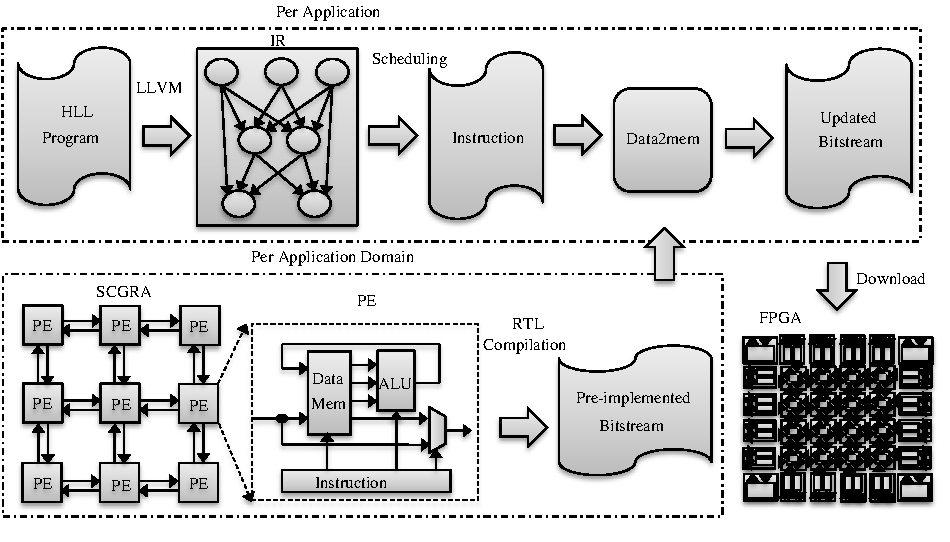
\includegraphics[width=0.85\linewidth]{design-flow}
\vspace{-1em}
\end{figure}

\textbf{Colin's work on the SCGRA based HLS}
\begin{itemize}
\item Operation scheduling
\item SCGRA design and implementation
\item Application specific SCGRA topology synthesis
\end{itemize}

\end{frame}

%------------------------------------------------
\begin{frame}[t]
\frametitle{Preliminary loop unrolling analysis}
\vspace{-1em}
\textbf{loop unrolling influence on performance and overhead}
\begin{figure}
\vspace{-1em}
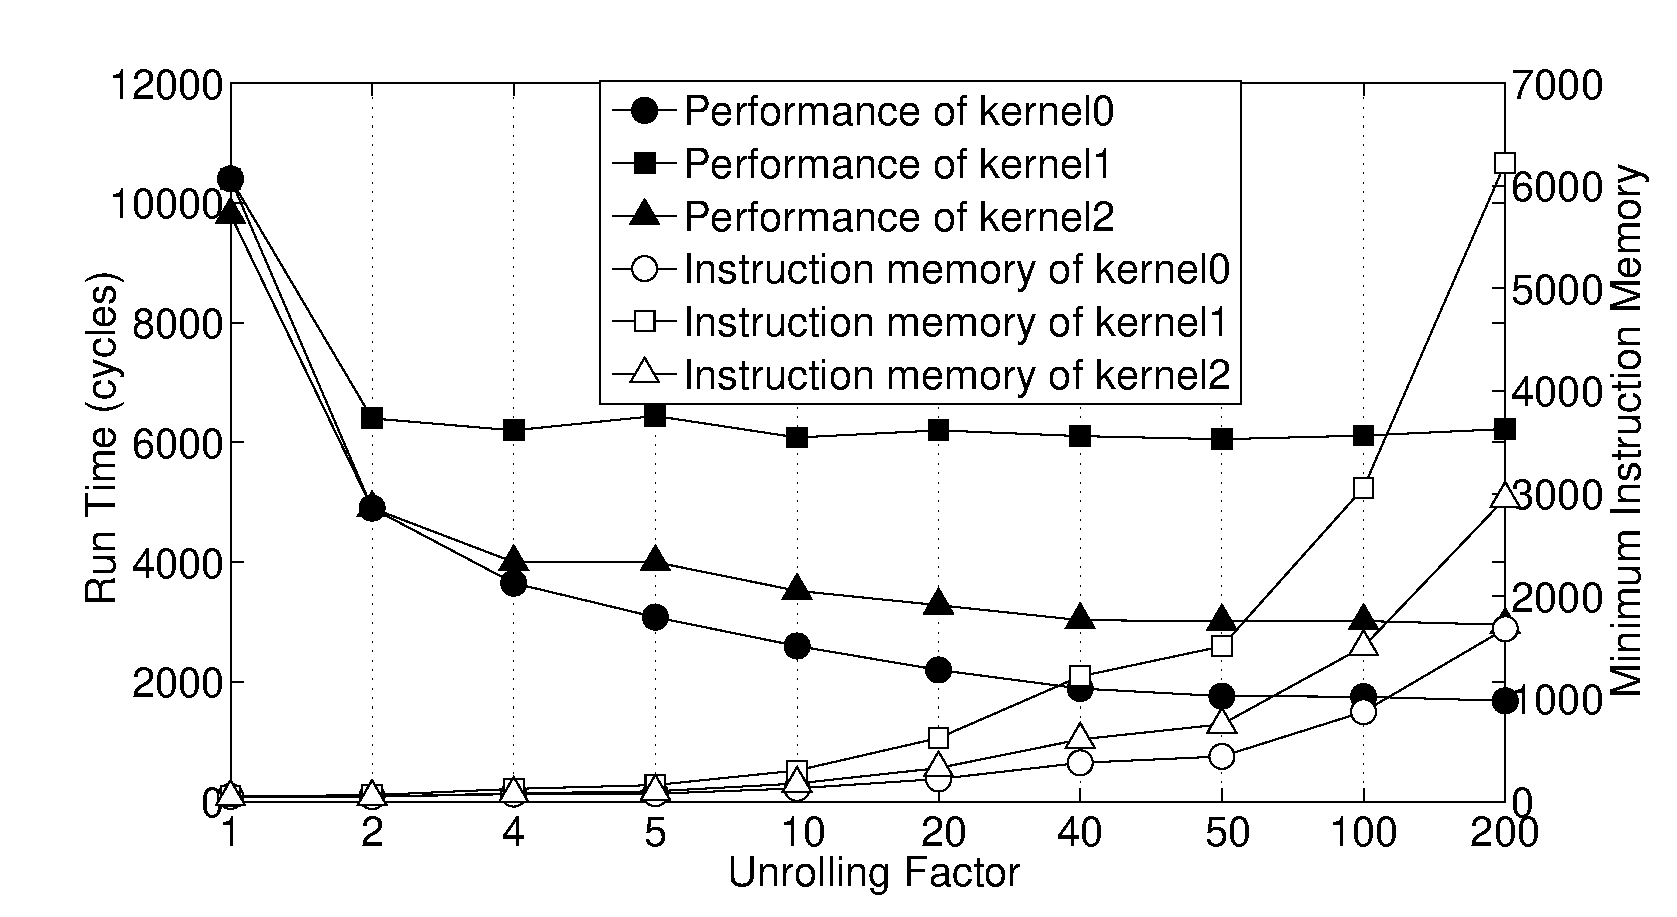
\includegraphics[width=0.6\linewidth]{loop-unrolling}
\vspace{-1em}
\end{figure}

\textbf{Irregular loop bound}
\begin{figure}
\vspace{-1em}
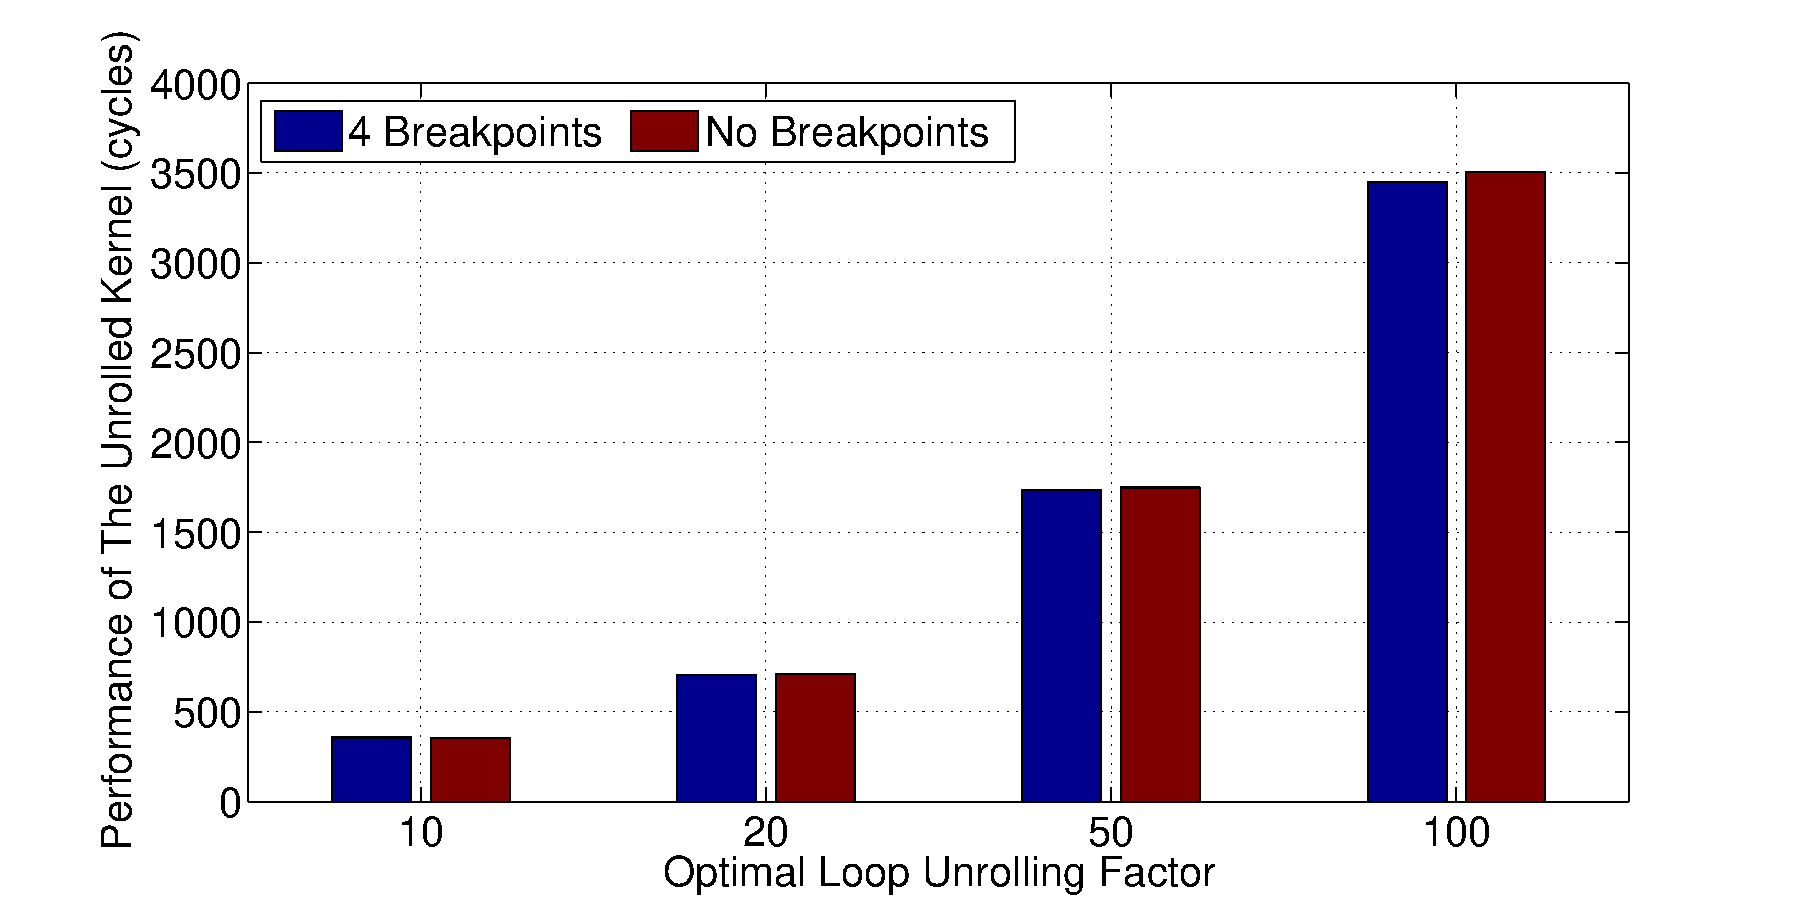
\includegraphics[width=0.6\linewidth]{any-loop-unrolling}
\vspace{-1em}
\end{figure}
\end{frame}

%------------------------------------------------
\begin{frame}[t]
\frametitle{HW/SW communication on Zedboard}

\textbf{Zedboard platform}
\begin{figure}
\includegraphics[width=0.7\linewidth]{zynq}
\end{figure}
\textbf{Different communication methods}
\begin{itemize}
\item Accelerator coherence port
\item Central DMA, Video DMA, XDMA
\item GPIO
\end{itemize}

\end{frame}

%------------------------------------------------
\section{Conclusion}
\begin{frame}[t]
\frametitle{Self-evaluation}

\textbf{About the progress and publciation}
\begin{itemize}
\item Didn't work hard enough
\item Didn't not balance well between the engineering work and research focus
\item Have taken 10 RPG courses up to now
\end{itemize}

\end{frame}

%------------------------------------------------

\end{document} 
